\documentclass[a4paper,12pt]{article}
\addtolength{\oddsidemargin}{-1.cm}
\addtolength{\textwidth}{2cm}
\addtolength{\topmargin}{-3cm}
\addtolength{\textheight}{3.5cm}
\makeindex


\usepackage[pdftex]{graphicx}
\usepackage{makeidx}
\usepackage{float}
\usepackage{hyperref}
\hypersetup{
	colorlinks=true,
	linkcolor=blue,
	filecolor=magenta,      
	urlcolor=cyan,
}



% define the title
\author{CodeBlox}
\title{Tender}
\begin{document}
	\setlength{\parskip}{6pt}
	
	% generates the title
	\begin{titlepage}
		\begin{center}
			
\includegraphics[width=1\textwidth]{./Pictures/up_logo.png}\\[1.5cm] 
			\textsc{\LARGE Department of Computer Science} \\ [.5cm]
			\textsc{\Large User Manual} \\ [.5cm]
			\line(1,0){450}\\[.5cm]
			\huge{\bfseries Client: Gavin Potgieter}\\
			\line(1,0){450}\\[.5cm]
			\textsc{\LARGE Team: CodeBlox}\\ [0.5cm]
			
			
			\textsc{\large Lethabo Mogase (Bsc: Computer Science)}\\
			\textsc{\large Lorenzo Spazzoli (Bsc: Computer Science)}\\
			\textsc{\large Bilal Muhammad (BIS: Multimedia)}\\
			\textsc{\large Dirk de Klerk (BIS: Multimedia)}\\ [3.9cm]
			
			\large\today
		\end{center}
	\end{titlepage}
	
	\tableofcontents
	\thispagestyle{empty}
	\footnotesize
	\normalsize
	
	
	
	
	\newpage
	\section{System Overview}
	The main objective of this system is to allow a delivery person into a demarcated area of your house when you are not there. You should be able to give access remotely and monitor the delivery person while you are not in the area. 
	The project has been named "DropOff" and has been persued by team CodeBlox.
	
	This document will demonstrate how the user would use the system.
	
	\section{System Configuration}
		
		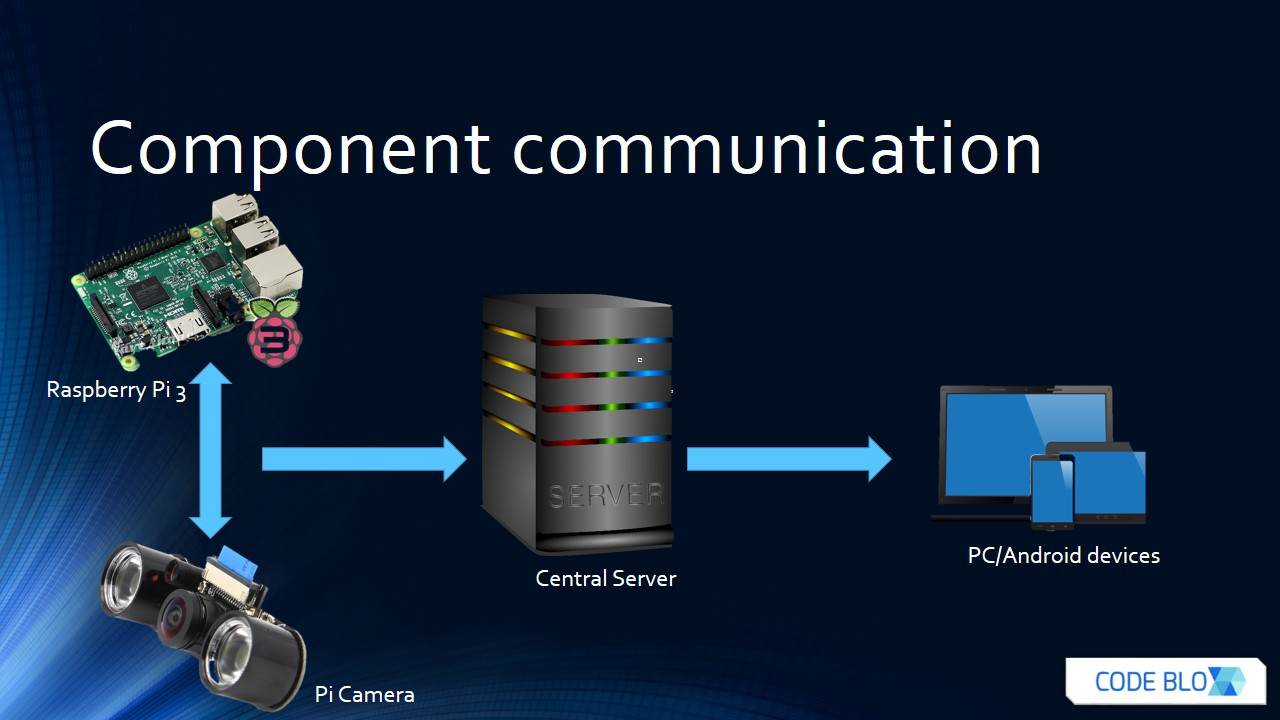
\includegraphics[width=1\textwidth]{./Pictures/CodeBlox.jpg}\\[1.5cm] 
	
		\subsection{Raspberry Pi 3}
		The Raspberry Pi is used to serve the purpose of the client. It handles all the requests passed down from the main server which include open/close gate, getting camera feed and handling other appliances in the system.
		
		\subsection{Pi Camera}
		The camera is simply used to stream a live video from the house to the owner.
		
		\subsection{Central Server}
		The central server is used to connect the user to their house from any location in the world as long as a live internet connection exists.
		
		\subsection{PC/Android devices}
		The live video is streamed to these devices and is also used as a remote to control the devices in the house.
		
	\section{Installation}
	
		\subsection{Software}
			\subsubsection{NodeJs}
			Install by using the following command: \newline
			\textbf{sudo apt-get install nodejs}
			\subsubsection{NPM(Node package manager)}
			We have used npm to install our node packages. It can be installed using: \newline
			\textbf{sudo apt-get install npm}
			\subsubsection{Installing dependencies}
			When working with nodejs, a package.json file is created whereby all the application dependencies are listed. The list for the dependencies can be found on our git repo at:
			\textbf{https://github.com/billibongers/CodeBlox---Main-Project/blob/master/Code/NodeJs\newline/personModule/package.json}
			\newline\newline
			To automatically install all dependencies run the command:\newline
			\textbf{npm install}
			\subsubsection{Installing application on andorid device}
			The android application is coded in Android Studio using pure java. It can be found in our Android git repo which is dedicated to the mobile app here:
			\textbf{https://github.com/lspazzoli\newline/CodeBlox-Android}
			\newline\newline
			The following is a graphical representation of how to install the application on a mobile phone once downloaded from the abovementioned URL
			
			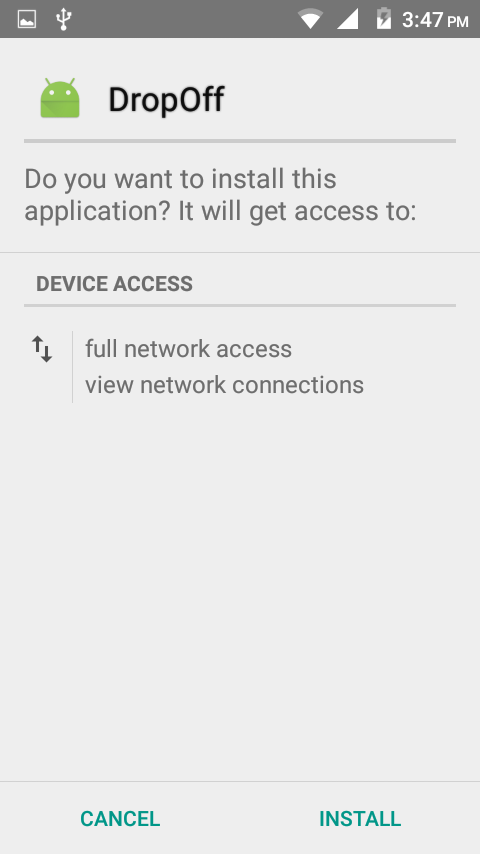
\includegraphics[width=10cm,height=10cm,keepaspectratio]{./Pictures/install1.png}
			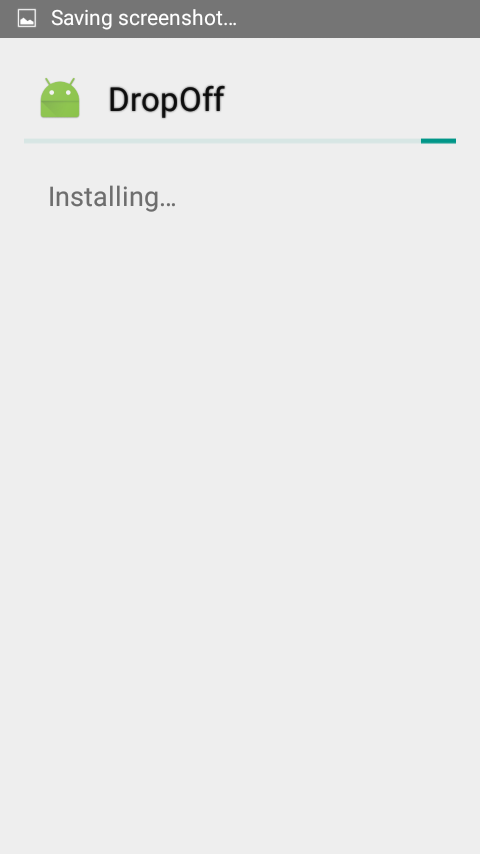
\includegraphics[width=10cm,height=10cm,keepaspectratio]{./Pictures/install2.png}
			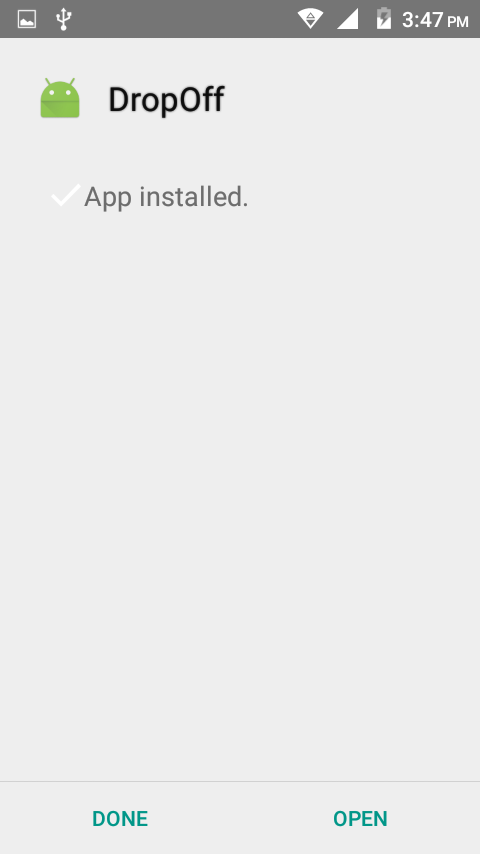
\includegraphics[width=10cm,height=10cm,keepaspectratio]{./Pictures/install3.png}\\
			Once the .apk has been clicked on, Step 1 appears telling you the permissions, these permissions are required to communicate with the pi and camera, they are networking permissions only. Step 2 installs the program and step 3 confirms the installation was successful\newline\newline
			
			\subsubsection{Application Information}
			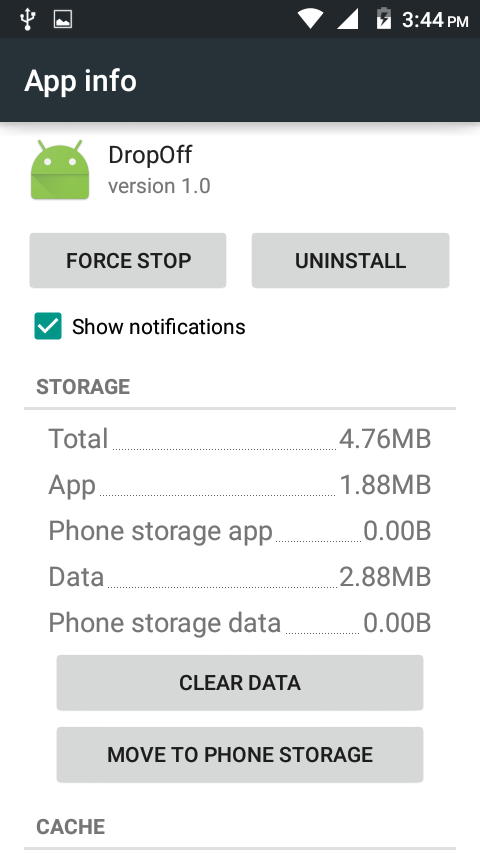
\includegraphics[width=10cm,height=10cm,keepaspectratio]{./Pictures/appinfo.png}\\
			The app is light weight, it uses less than 10mb of internal storage, this is so that it may run on low cost devices. The current version is 1.0 this is because the application has just entered its beta stages for the demo 2. The version 0.x was used for alpha and 2.x will be used for the actual release
			
			\subsubsection{Application Features}
			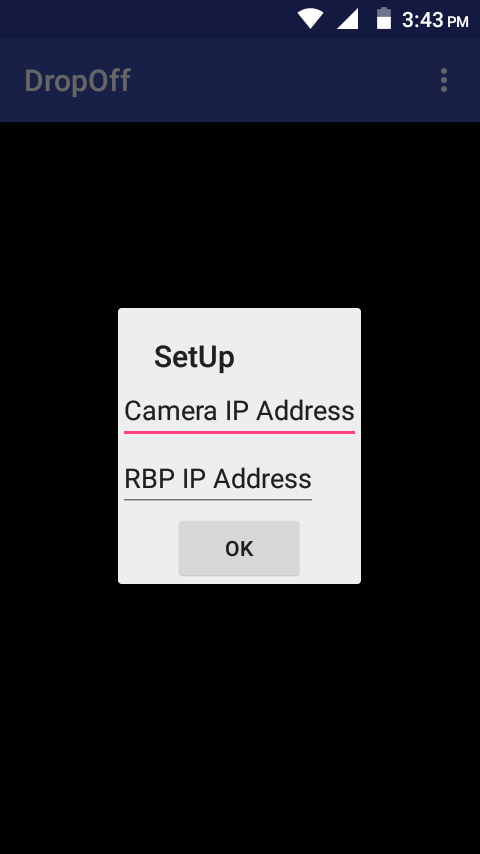
\includegraphics[width=10cm,height=10cm,keepaspectratio]{./Pictures/a1.png}
			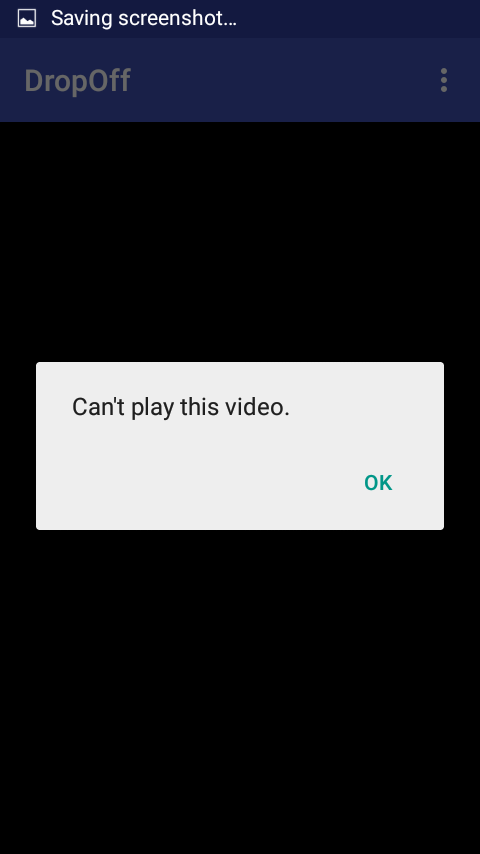
\includegraphics[width=10cm,height=10cm,keepaspectratio]{./Pictures/a2.png}
			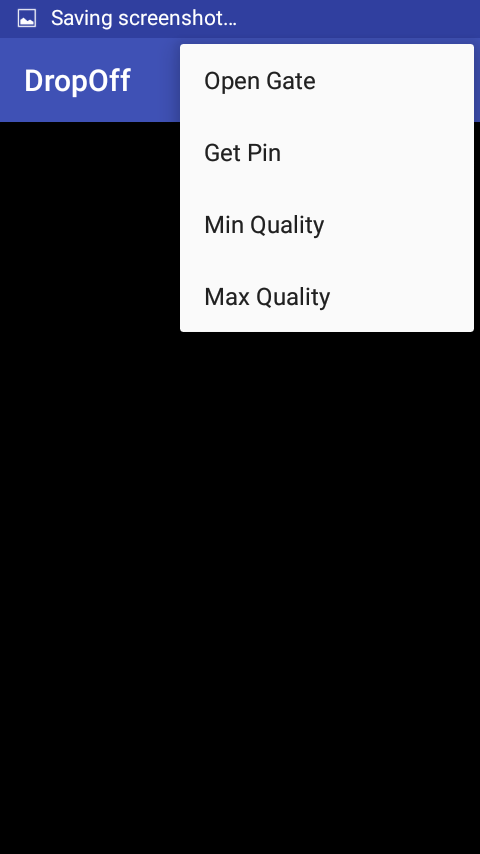
\includegraphics[width=10cm,height=10cm,keepaspectratio]{./Pictures/a3.png}\\
			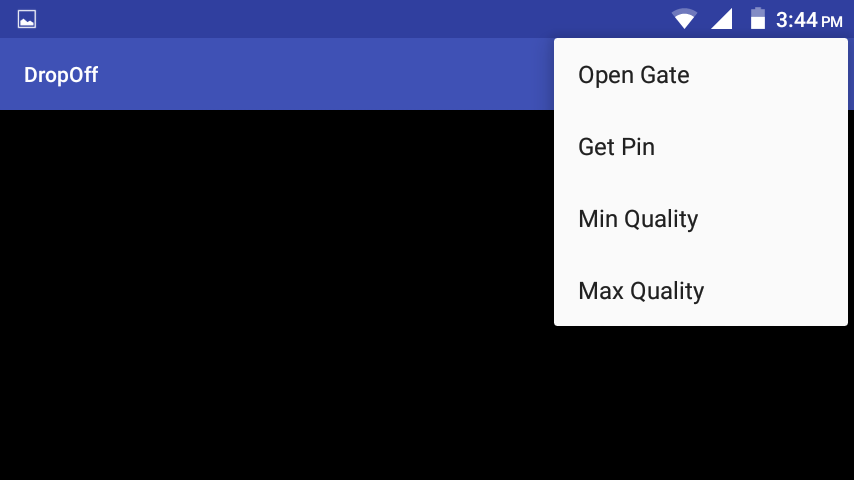
\includegraphics[width=10cm,height=10cm,keepaspectratio]{./Pictures/a4.png}
			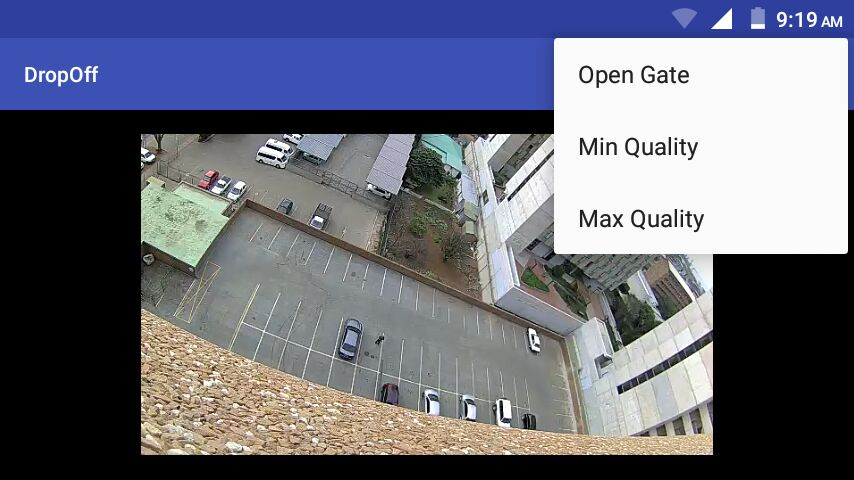
\includegraphics[width=10cm,height=10cm,keepaspectratio]{./Pictures/a5.jpg}\\ \newline
			\textbf{Screenshot1} Shows the beta version of the application as it is open here you enter the IP address of the pi and the IP camera, this is just for portability until we have an external server set up.\newline
			\textbf{Screenshot2} Displays the error messages associated with the connection to the camera being unsuccessful\newline
			\textbf{Screenshot3} Displays the option menu, this is triggered by clicking on the menu button on your device or clicking on the physical menu\newline
			\textbf{Screenshot4} shows the application with a feed working, this is application version 0.8, added from this point was the functionality as seen in screenshot 1 , the ability to get a pin from the raspberry pi and all errors that caused the app to crash have been resolved\newline 
			\textbf{Screenshot5} displays the application menu in landscape form\newline
			
		
				
		\subsection{Hardware}
	\section{Getting Started}
	
	\section{Using the system}
	
	\section{Troubleshooting}
	

\end{document}